\chapter{Related work}
\label{chap:rel_work}

We conducted a literature study to learn more about the state of the art in the semantic web and existing research on public transport route planners and their role in the semantic web.

We started with the related thesis of Jeroen Flipts \cite{Flipts2020}. He created a serverless route planner based on the \acrfull{csa} \cite{csa}. The thesis gives us the idea of implementing the \acrfull{raptor} algorithm \cite{Delling2014Oct}.

Since RAPTOR has some advantages over CSA, such as no preprocessing, good query times and Pareto optimal journeys out of the box, we hope to get an improved serverless route planner. These advantages made RAPTOR widespread, and the algorithm was quickly adopted in OpentripPlanner \cite{raptorinopentripplanner}.

\section{Public Transport Algorithms}
\begin{figure}[H]
    \centering
    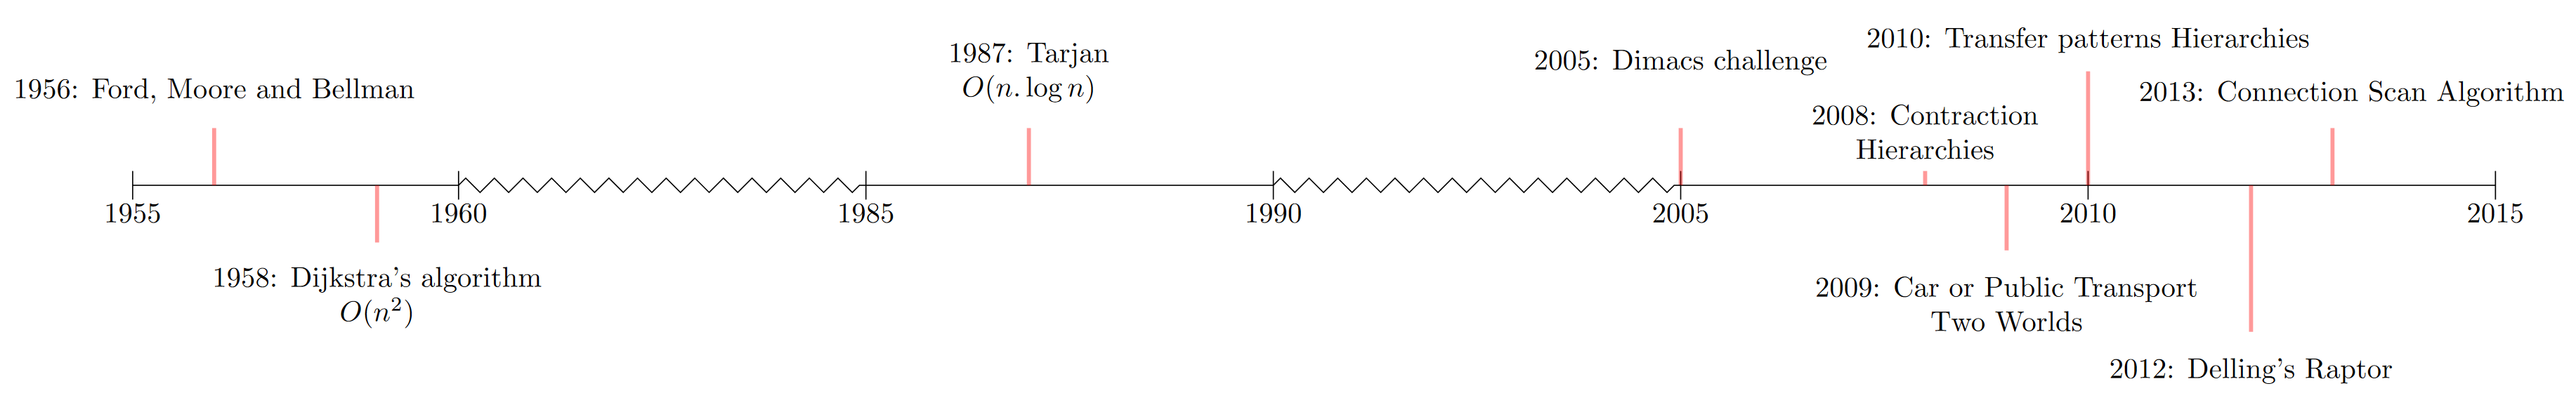
\includegraphics[width=\textwidth]{images/timeline.png}
    \caption{Timeline describing the developments in route planning. The crossed parts represents }
    \label{fig:timeline}
\end{figure}
In \autoref{fig:timeline} the history of the 
\subsection{Transfer patterns}
It described a method using a journey planning algorithm to pre-calculate all the unique journeys for the entire graph. This means when a real-time query comes in we can just look up the schedule that matches that journey.
% IDEA, HYDRIDE? Calculate for IC's , for the rest raptor? It is quick to calculate if a station has an IC Passing through it.
\subsection{\acrfull{csa}}
\subsection{\acrfull{raptor}}
RAPTOR is a graph-based algorithm which solves queries in rounds. Round K computes the fastest way of getting to every stop with at most k - 1 transfers or k trips.

\begin{enumerate}
    \item Each node gets a multilabel. $(\tau_0,...,\tau_k)$ with $\tau_i$ representing the earliest arrival time in $i$ trips. We init all arrival times in each label with $\infty$. Except for the departing node, where $\tau_0$ is set to the depart time of our search criteria.
    \item For each round $k$ our goal is to compute $\tau_k$. This happens in three stages:\begin{enumerate}
        \item Set the earliest arrival time k ($\tau_k$) to that of iets predescor ($\tau_{k-1}$). This is an upper bound since we are not interested in slower stop times than the previous round.
        \item We iterate over the routes. We calculate for each stop $p$ on the route $r$, the earliest trip we can take. This does not always exist. We search stops along the route $r$ that has the earliest trip $t$. This means we can hop on the route $r'$ in $p$. For subsequent stops in $r'$, we can update $\tau_k$ according to the found trip $t$.
        \item Finally, footpaths are considered. We check if $\tau_k$ can be improved by using a footpath between two stops. 
    \end{enumerate}
\end{enumerate}

\begin{figure}[H]
    \centering
    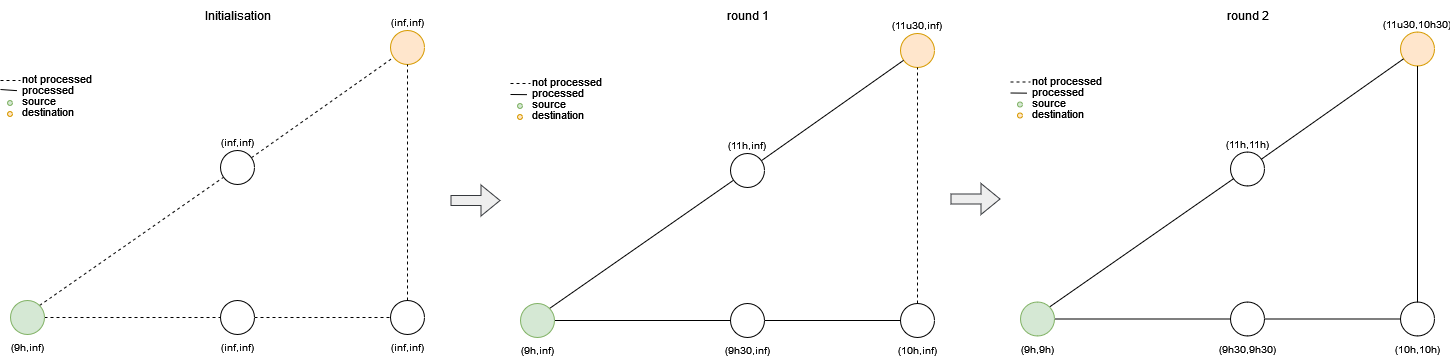
\includegraphics[width=\textwidth]{images/rqptor.drawio.png}
    \caption{A small example using raptor, two rounds are shown }
    \label{fig:enter-label}
\end{figure}

\subsection{Ontology}

A small study was conducted to find an ontology that best suited our needs. Many of the studied ontologies for transport are focused on specific use cases, for example, urban freight \cite{BOUHANA20153724}. They do not have a broad domain. 

A relatively old ontology designed to use with a user planning tool based on journey patterns \cite{5507372} was found and could support RAPTOR. Interestingly, they implemented a mobile application to plan tourist bus routes, but it relied on server-side queries. Other downsides are that there is no multi-modal support (only transport by bus) and no multi-operator support. The ontology was not directly available from the authors.

Using the survey of transportation ontologies \cite{Katsumi2018Apr}, we only identify three ontologies that support journey patterns. Two are focused on city logistics and urban systems, a different domain. The last ontology (Transportation ontology for content personalization) applies to PT, but the ontology is not directly available.

%transmodel ontology
Every PT agent is required by European directives to be compatible with Transmodel, so an ontology aligned with Transmodel is interesting. Further, the Transmodel ontology supports journey patterns. However, the ontology could be too broad, which leads to several potential problems. For example, it can make it hard to find relevant information, as the ontology may contain too many concepts and relationships that are not relevant. Furthermore, as the ontology may not be compatible with other ontologies used in those sources, integration from different sources can also be challenging.

%OSLO Mobiliteit: Dienstregeling en Planning
The last ontology we looked at is the "OSLO Mobiliteit - Dienstregeling en Planning" \cite{osloflanders} ontology. The ontology is developed by Open Standaarden voor Linkende Organisaties (OSLO), a department of Data Flanders. It has been based on the EPIP profile of NETEX. NETEX is based directly on Transmodel, so the ontology has some similarities with the Transmodel ontology but is less broad than the Transmodel ontology.

\begin{landscape}
\begin{table}[]
\centering
\begin{tabular}{|l|l|l|l|l|l|l|}
\hline
\textbf{Ontology} &
  \textbf{\begin{tabular}[c]{@{}l@{}}Journey\\ patterns?\end{tabular}} &
  \textbf{\begin{tabular}[c]{@{}l@{}}Multi-\\ modal?\end{tabular}} &
  \textbf{\begin{tabular}[c]{@{}l@{}}Multi-\\ operator?\end{tabular}} &
  \textbf{\begin{tabular}[c]{@{}l@{}}Designed for use\\  with routeplanners\end{tabular}} &
  \textbf{\begin{tabular}[c]{@{}l@{}}directly available\\  for reuse?\end{tabular}} &
  \textbf{DOI} \\ \hline
\begin{tabular}[c]{@{}l@{}}Intoducing the public transport\\ domain to the web of data\end{tabular} &
  yes &
  yes &
  yes &
  yes &
  no &
  10.1007/978-3-319-11746-1\_38a \\ \hline
iCity Ontology &
  yes &
  no &
  no &
  no, urban systems &
  yes, Github &
  w3id.org/icity/iCityOntology\_v1\_Report.pdf \\ \hline
Genclon &
  yes &
  no &
  no &
  no, city logistics &
  no &
  10.1016/j.eswa.2012.03.068 \\ \hline
\begin{tabular}[c]{@{}l@{}}Transportation ontology\\ for content personalization\end{tabular} &
  yes &
  yes &
  yes &
  yes &
  no &
  10.1016/j.eswa.2012.12.028 \\ \hline
Transmodel ontology &
  yes &
  yes &
  yes &
  yes &
  yes, Github &
  10.3233/SW-210451 \\ \hline
OSLO Ontology &
  yes &
  yes &
  yes &
  yes &
  yes &
  / \\ \hline
\end{tabular}
\caption{}
\label{tab:my-table}
\end{table}
\end{landscape}